\documentclass[11pt,a4paper]{article}

\usepackage[margin=2.2cm]{geometry}
\usepackage[T1]{fontenc}
\usepackage{lmodern}
\usepackage{amsmath}
\usepackage{graphicx}
\usepackage{booktabs}
\usepackage{caption}
\usepackage{siunitx}
\usepackage[hidelinks]{hyperref}
\captionsetup{font=small,labelfont=bf}
\graphicspath{{figures/}}

\title{Does Rain Change How NYC Taxi Passengers Tip?\\
\large Evidence from 29 Million Trips in 2024}
\author{Your Name\\\small\url{https://github.com/khanhlinh-dang/<repository>}}
\date{}

\begin{document}
\maketitle

\begin{abstract}
\noindent
I study whether rain at pickup changes the tipping behaviour of New York City Yellow Taxi passengers. A pilot on
one month of data (April 2024) found no significant difference between rainy and dry days, but a power analysis
shows it could only detect very large effects. The main study therefore uses all \num{29.4} million card-paid
trips of 2024, matches each trip to the precipitation in its pickup hour, and estimates the effect of rain with
regression that controls for time, trip characteristics and temperature, with standard errors clustered by day.
A rainy hour changes the tip rate by $+0.017$ percentage points (95\% CI $[-0.018, 0.051]$) on a mean of
17.8\%, a precisely estimated null that survives all robustness checks. A naive comparison suggests a small
positive effect, but this is explained by when rain falls, and a lower dollar tip on rainy days is fully
explained by shorter trips. A plausible mechanism is the payment screen's default: 46\% of card trips tip exactly
20\% of the pre-tip total.
\end{abstract}

\section{Introduction}
Tipping is a voluntary payment, which makes it a natural test of how situational factors shape generosity.
Weather is a candidate factor with two opposite predictions. Passengers might tip \emph{more} in the rain, out of
gratitude for a ride when taxis are hard to find \cite{farber2015}, or \emph{less}, because the trip is slower
and less pleasant. Previous work on New York taxis links sunshine to higher tips \cite{devaraj2017} and shows
that the default tip suggestions on the payment screen strongly shape what passengers pay \cite{haggag2014}.

This project asks: \emph{holding time and trip characteristics fixed, does rain at pickup change the share of
the bill that passengers tip?} It contributes (i)~an analysis of a full year of trips with rain measured at the
\emph{hour} of pickup rather than the day, (ii)~an explicit treatment of confounding and of the difference
between statistical and practical significance, and (iii)~evidence that the tip default limits how much weather
can matter.

\section{Data}
\paragraph{Trips.} I use the NYC Taxi \& Limousine Commission Yellow Taxi trip records for January--December
2024 \cite{tlc}, which contain \num{41.2} million trips. I keep trips paid by credit card, because cash tips are
not recorded and would appear as false zeros. I also keep only standard-rate and JFK flat-fare trips, fares of at
least \$3, distances of 0--100 miles, durations of 1--180 minutes, and tips between 0 and 100\% of the pre-tip
total. The final sample has \num{29393010} trips (71.4\% of the raw data). Most of the loss comes from the
card-payment rule (26\%).

\paragraph{Outcome.} The tip rate is the tip as a percentage of the \emph{pre-tip total} (fare, surcharges and
tolls). This is the amount on the payment screen and the base for its suggested tips. Figure~\ref{fig:dist}
shows that this is the correct base: tips bunch sharply at 20\%, 25\% and 30\% of the pre-tip total, while
relative to the fare alone the same spikes are smeared out. 46.4\% of all card trips tip exactly 20\% to the
cent, and 4.1\% tip nothing. The mean tip rate is 17.8\% (\$4.29).

\paragraph{Weather.} Hourly precipitation and temperature at the Central Park grid point come from the ERA5
reanalysis \cite{era5} via the Open-Meteo API. Because reanalysis is a model estimate, I validate it against the
NOAA GHCN-Daily rain gauge in Central Park \cite{ghcn}. The daily totals correlate at $r=0.83$, and the two
sources agree on 88.8\% of rainy-day labels ($\geq 1$\,mm). An hour is \emph{rainy} if it records at least
0.25\,mm (0.01\,in, the standard threshold for measurable precipitation); 9.0\% of trips start in a rainy hour.

\begin{figure}[t]
  \centering
  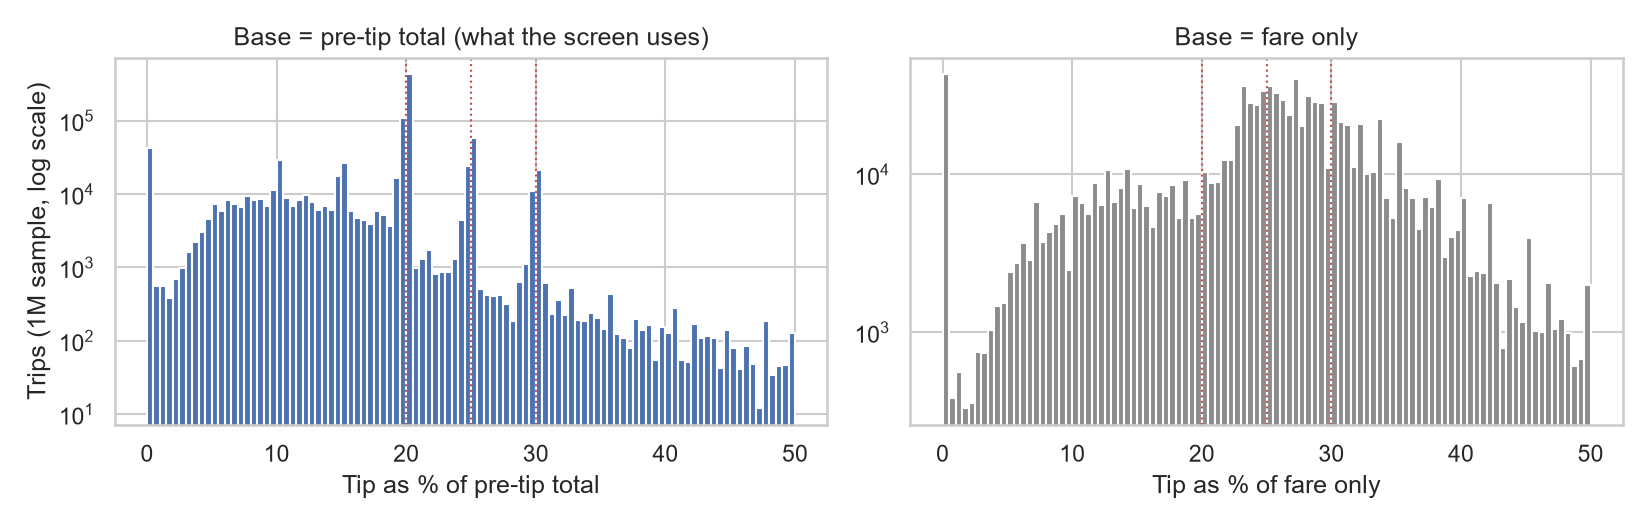
\includegraphics[width=\linewidth]{02_tip_pct_distribution.png}
  \caption{Distribution of tip rates (1M-trip sample, log scale). Relative to the pre-tip total (left), tips
  bunch at the preset buttons; relative to the fare alone (right), they do not.}
  \label{fig:dist}
\end{figure}

\section{Methods}
\paragraph{Pilot.} For April 2024 I estimate a 95\% confidence interval for the mean tip from a random sample of
\num{5000} trips. Because tips are right-skewed, the $t$-interval is checked against a percentile bootstrap.
Rainy and dry days are compared with Welch's $t$-test and the Mann--Whitney $U$ test, with Cohen's $d$ as the
effect size.

\paragraph{Day-level analysis.} The same tests are repeated with all 366 days, using the station's daily rain.
A $\chi^2$ test checks whether rainy days are evenly spread across months and weekdays. A day-level OLS
regression then adds weekday and month fixed effects, a holiday dummy and temperature (HC3 standard errors). A
second specification also adds the day's mean log distance and duration (the \emph{trip mix}).

\paragraph{Trip-level regression.} The main model is
\begin{equation}
  \text{tip}_i = \beta\,\text{rain}_{h(i)} + \alpha_{\text{hour}(i)} + \gamma_{\text{dow}(i)} +
  \delta_{\text{month}(i)} + \mathbf{x}_i'\boldsymbol{\eta} + \varepsilon_i,
\end{equation}
where $\text{rain}_{h(i)}$ indicates rain in the pickup hour, and $\mathbf{x}_i$ contains a holiday dummy,
temperature, log distance, log duration, an airport indicator, the JFK flat fare and the passenger count.
Trips on the same day share the same weather and unobserved shocks, so standard errors are clustered by day (366
clusters) \cite{cameron2015}. Treating trips as independent would understate the uncertainty by a large factor.
For computational convenience, the model is estimated on a random sample of 3 million trips. A second
independent sample gives the same result. I also estimate linear probability models for tipping at all and for
tipping exactly 20\%, and the tip-rate model among tippers only.

\section{Results}
\paragraph{Pilot.} The mean tip is \$4.31 (95\% CI $[\$4.20, \$4.42]$), and the bootstrap interval is
$[\$4.20, \$4.42]$. Rainy and dry days do not differ (Welch $p=0.47$, $d=-0.27$). With 15 vs.\ 15 days,
however, the test has 80\% power only for effects of $d \geq 1.06$. The pilot is therefore uninformative about
moderate effects.

\paragraph{Full year, day level.} With 105 rainy and 261 dry days (minimum detectable $d=0.32$), the mean tip
\emph{rate} does not differ ($+0.03$\,pp, Welch $p=0.33$). The mean \emph{dollar} tip, however, is lower on rainy
days ($-\$0.08$, $p=0.002$, $d=-0.37$). Rainy days are not evenly spread over the year ($\chi^2_{11}=30.0$,
$p=0.002$; e.g.\ 48\% of days in January and December but none in October), which motivates the regression
controls. With calendar controls, the dollar gap shrinks to $-\$0.045$ ($p=0.009$). Adding the day's trip mix
removes it entirely ($+\$0.003$, $p=0.52$). Rainy days have shorter trips with smaller dollar tips, but
passengers do not tip a smaller \emph{share}. This is a composition effect, not a change in behaviour.

\begin{table}[t]
\centering
\small
\caption{Trip-level effect of rain in the pickup hour. OLS / linear probability models on 3M trips; SE clustered
by day. All models except (1) include the full set of controls.}
\label{tab:main}
\begin{tabular}{llS[table-format=-1.3]cc}
\toprule
& Outcome & {Coef.} & 95\% CI & $p$ \\
\midrule
(1) & Tip rate (pp), no controls      &  0.090 & $[0.031,\ 0.150]$   & 0.003 \\
(2) & Tip rate (pp)                   &  0.017 & $[-0.018,\ 0.051]$  & 0.343 \\
(3) & P(tip $>$ 0)                    & -0.001 & $[-0.002,\ -0.000]$ & 0.029 \\
(4) & Tip rate (pp), tippers only     &  0.039 & $[0.005,\ 0.073]$   & 0.023 \\
(5) & P(tip = exactly 20\%)           & -0.005 & $[-0.007,\ -0.002]$ & $<0.001$ \\
\bottomrule
\end{tabular}
\end{table}

\paragraph{Main result.} Table~\ref{tab:main} reports the trip-level estimates. Without controls (1), rainy hours
show a small positive and significant effect. With controls (2), the estimate falls by 80\% to $+0.017$\,pp and
is not significant. The 95\% confidence interval excludes effects larger than 0.05\,pp, or 0.3\% of the mean tip
rate. The extra controls thus remove confounding by \emph{when} it rains, and what remains is a precisely
estimated null. Figure~\ref{fig:robust} shows that this holds across rain thresholds from 0.1 to 2.5\,mm/h, the
station-based daily definition, the exclusion of airport trips and a second random sample. A continuous intensity
measure ($+0.003$\,pp per mm/h, $p=0.64$) agrees.

\paragraph{Margins.} Models (3)--(5) show that rain slightly reduces the probability of tipping exactly 20\%
($-0.5$\,pp on a base of 46\%) and slightly raises the tip rate among tippers ($+0.04$\,pp). These effects are
statistically detectable only because of the sample size. Their magnitudes are about 1\% of the baseline or
less, so they are practically negligible. Given the number of outcomes tested, I do not interpret them as
substantive findings.

\begin{figure}[t]
  \centering
  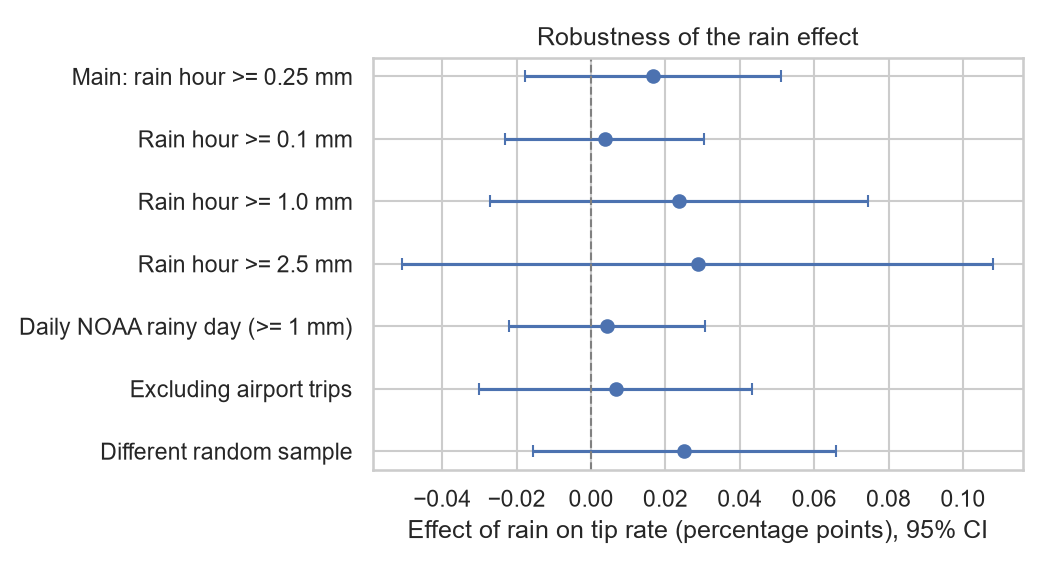
\includegraphics[width=0.72\linewidth]{02_robustness.png}
  \caption{Effect of rain on the tip rate under alternative specifications (95\% CI, SE clustered by day).}
  \label{fig:robust}
\end{figure}

\section{Discussion and limitations}
Rain has no economically meaningful effect on NYC taxi tipping in 2024. The most plausible explanation is the
strength of the default: almost half of all passengers press the 20\% button, which leaves little room for
situational factors to act. This is consistent with \cite{haggag2014}. The analysis also shows two common
pitfalls. A naive comparison is confounded by the timing of rain, and an aggregate difference in dollar tips
reflects a change in \emph{which} trips are taken rather than how individuals behave.

The study has limitations. Only card trips are observed, and cash payers may tip differently. Rain is measured
at a single grid point, so local rain elsewhere in the city adds measurement error that biases estimates towards
zero, although the station validation is reassuring. The design is observational, so unobserved factors
correlated with rain, such as cancelled events, cannot be excluded. Natural extensions are to use zone-level
rainfall radar data, to compare with For-Hire Vehicle (Uber/Lyft) trips whose apps use different defaults, and
to use the 2024 data as a pre-registered benchmark for other years.

\section*{Reproducibility}
All code, the data-download script and fixed random seeds are available in the repository. The full pipeline
runs in about 30 minutes on a laptop with 8\,GB of RAM.

\begin{thebibliography}{9}
\bibitem{cameron2015} A.~C. Cameron and D.~L. Miller. A practitioner's guide to cluster-robust inference.
  \emph{Journal of Human Resources}, 50(2):317--372, 2015.
\bibitem{devaraj2017} S.~Devaraj and P.~C. Patel. Taxicab tipping and sunlight. \emph{PLOS ONE},
  12(6):e0179193, 2017.
\bibitem{farber2015} H.~S. Farber. Why you can't find a taxi in the rain and other labor supply lessons from cab
  drivers. \emph{Quarterly Journal of Economics}, 130(4):1975--2026, 2015.
\bibitem{haggag2014} K.~Haggag and G.~Paci. Default tips. \emph{American Economic Journal: Applied Economics},
  6(3):1--19, 2014.
\bibitem{era5} H.~Hersbach et~al. The ERA5 global reanalysis. \emph{Quarterly Journal of the Royal
  Meteorological Society}, 146(730):1999--2049, 2020.
\bibitem{ghcn} M.~J. Menne, I.~Durre, R.~S. Vose, B.~E. Gleason, and T.~G. Houston. An overview of the Global
  Historical Climatology Network-Daily database. \emph{Journal of Atmospheric and Oceanic Technology},
  29(7):897--910, 2012.
\bibitem{tlc} NYC Taxi \& Limousine Commission. TLC Trip Record Data.
  \url{https://www.nyc.gov/site/tlc/about/tlc-trip-record-data.page}, accessed 2026.
\end{thebibliography}

\end{document}
